
%(BEGIN_QUESTION)
% Copyright 2011, Tony R. Kuphaldt, released under the Creative Commons Attribution License (v 1.0)
% This means you may do almost anything with this work of mine, so long as you give me proper credit

Tre nivåinstrumenter måler samme væskenivå i bunnen av dette fraksjoneringstårnet (LT-38a, LT-38b og LT-38c), men målingene deres er ikke enige. En operatør ber deg undersøke saken, og viser på kontrollsystemet at LT-38a viser 34.8\%, LT-38b viser 35.1\% og LT-38c viser 40.4\%. I henhold til P\&ID er LT-38a hydrostatisk (måler trykk via to fjernmembraner), LT-38b er et radarinstrument (måler nivå via refleksjonstid for en radarbølge inne i et kammer), og LT-38c er magnetostriktivt (måler posisjonen til en flottør i et annet kammer). Den visende regulatoren (LIC-38) viser et nivå på 35.1\%:

$$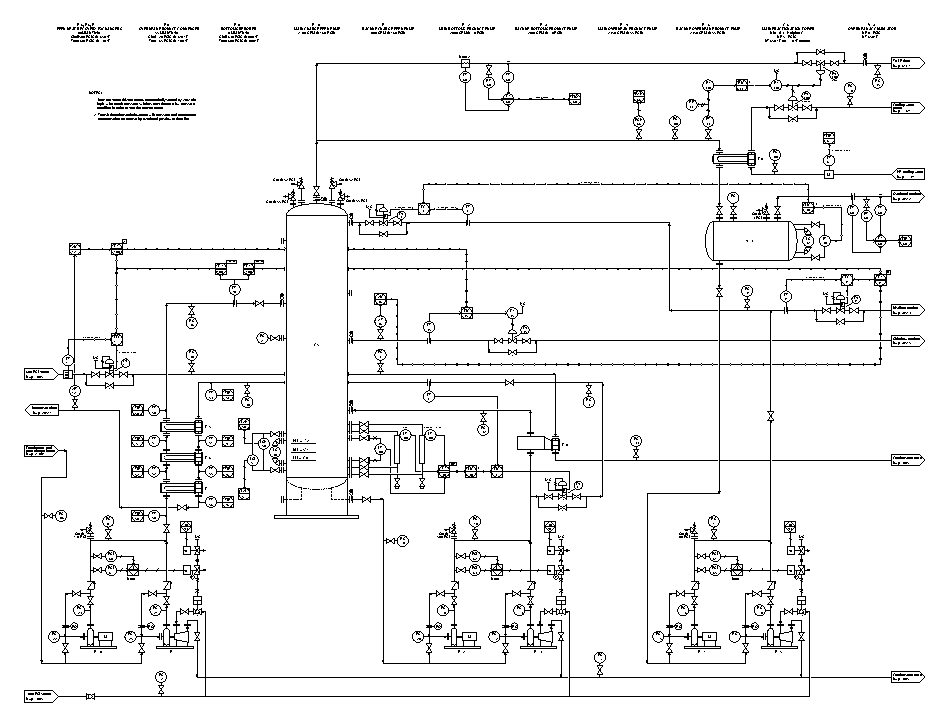
\includegraphics[width=15.5cm]{i0001rx01.eps}$$

Basert på informasjonen du har, identifiser en tilstand som kan forklare avviket mellom disse transmitterindikasjonene, og bestem også hva første diagnostiske steg bør være.

\vskip 20pt \vbox{\hrule \hbox{\strut \vrule{} {\bf Forslag til sokratisk diskusjon} \vrule} \hrule}

\begin{itemize}
\item{} Hvorfor tror du det brukes tre ulike instrumenter for å måle samme væskenivå i denne applikasjonen?
\item{} Identifiser funksjonen til LY-38.
\end{itemize}

\underbar{file i01200}
%(END_QUESTION)





%(BEGIN_ANSWER)

Et enkelt diagnostisk steg er å endre settpunktet til regulator LIC-38 (i automatisk modus) med 5\% eller 10\%, for å se om {\it alle tre} transmitterne viser nivåendring, eller bare de to som er mest enige.

%(END_ANSWER)





%(BEGIN_NOTES)

En sannsynlig feil er at flottøren i LT-38c rett og slett har satt seg fast. Nesten alle former for kalibreringsfeil (f.eks. nullpunktsforskyvning, spennforskyvning, ikke-linearitet osv.) i LT-38c er også plausible.



\vskip 20pt \vbox{\hrule \hbox{\strut \vrule{} {\bf Virtuell feilsøking} \vrule} \hrule}

Denne oppgaven egner seg godt som en ``Virtuell feilsøking''-øvelse. Når du presenterer diagrammet for elevene, tenker du først ut en bestemt feil i systemet. Deretter presenterer du ett eller flere symptomer på denne feilen (noe en operatør eller annen bruker av systemet kan observere). Elevene foreslår deretter ulike diagnostiske tester på systemet for å identifisere type feil og hvor den sitter, som om de var teknikere som feilsøker problemet. Din oppgave er å fortelle hva resultatet ville vært for hver foreslåtte diagnostiske test, og dokumentere resultatene slik at alle elevene kan se dem.

Under og etter øvelsen er det nyttig å stille oppfølgingsspørsmål til elevene, for eksempel:

\begin{itemize}
\item{} Hva forteller resultatet av den siste diagnostiske testen deg om feilen?
\item{} Anta at resultatet av den siste diagnostiske testen var annerledes. Hva ville det i så fall fortalt deg om feilen?
\item{} Er den siste diagnostiske testen den beste vi kunne gjort?
\item{} Hva ville vært den ideelle rekkefølgen på testene for å diagnostisere problemet med færrest mulig trinn?
\end{itemize}

%INDEX% Measurement, level: troubleshooting
%INDEX% Process: distillation, generic (realistic P\&ID shown)

%(END_NOTES)
